\section{Zielsetzung}
Das Ziel der Arbeit ist es eine konkrete Programmiersprache anhand von wenigen Vorgaben zu definieren. Anschließend soll ein Compiler für die definierte Sprache entwickelt werden. Dieser Compiler muss in der Lage sein ein vom Benutzer entworfenes Programm auf Fehler zu prüfen, gegebenenfalls Fehler auszugeben und letztendlich eine ausführbare Datei für die \ac{jvm} zu erzeugen. In der \cref{pic:CompilerAufbau} ist der Grundlegende Aufbau eines Compilers zu sehen, und damit die einzelnen Bestandteile, welche Umgesetzt werden müssen.

\begin{figure}[h!]
	%\includegraphics[width=1\textwidth]{content/pictures/LoRaWAN-OSI.JPG}
	\centering
	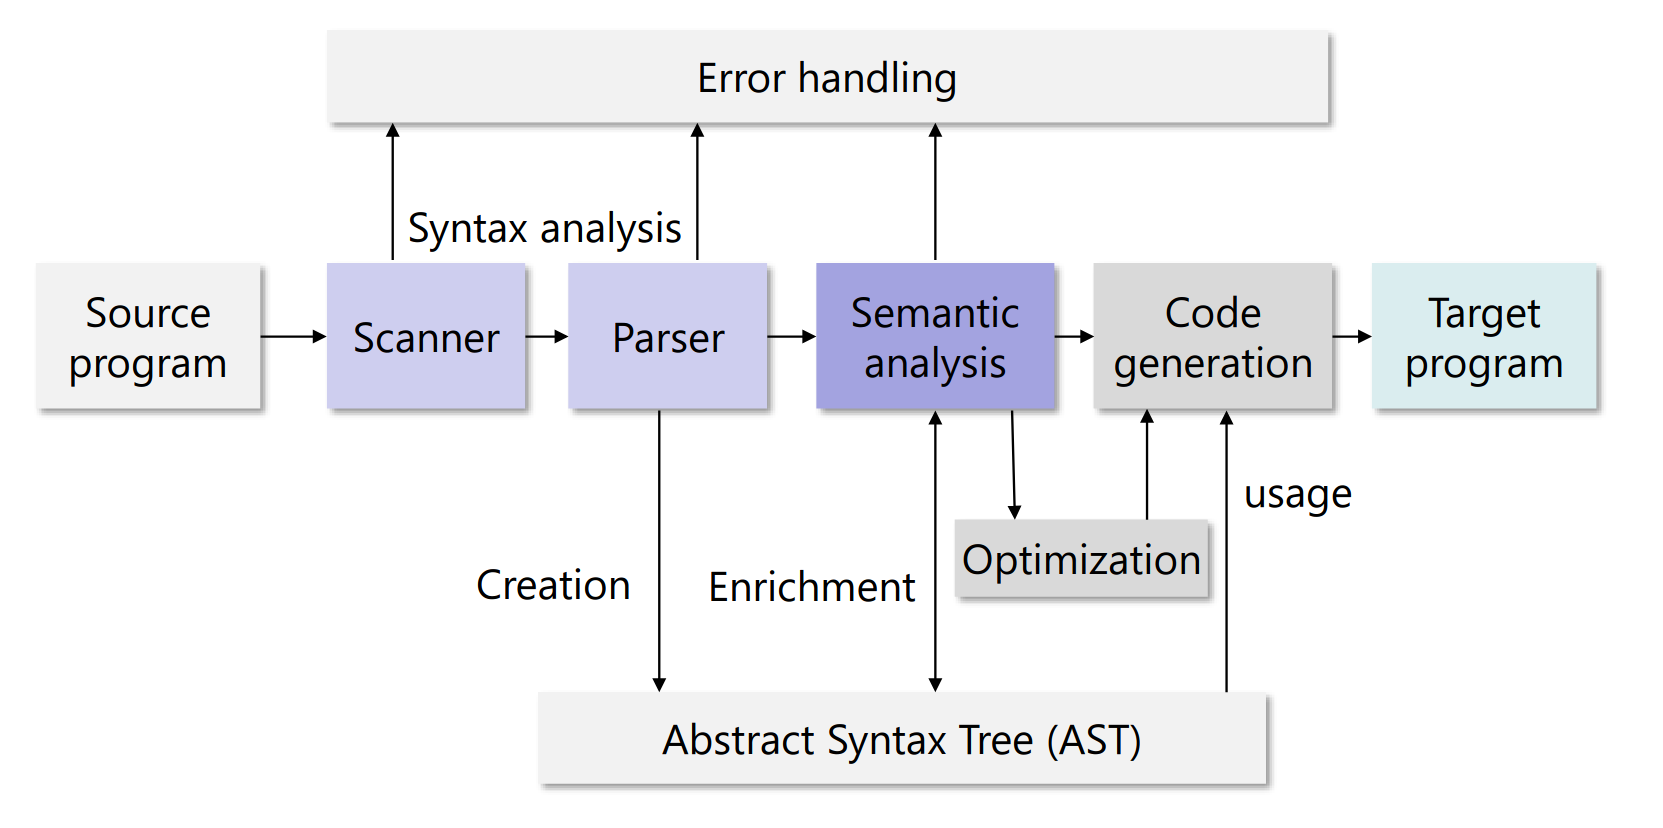
\includegraphics[width=12cm]{content/pictures/compiler.png}
	\captionsource{Aufbau eines Compilers}{\cite[S. 5]{GottfriedVossen2016}}
	%	\source{\cite[S. 5]{SemtechCorporation.2020}}
	\label{pic:CompilerAufbau}
\end{figure}

Anschließend soll für die entwickelte Programmiersprache eine IDE Integration erfolgen, um den Nutzer bei der Entwicklung von Programmen mit Features wie Syntax-Highlight zu unterstützen.

Nachdem Verständnis für die Funktionsweise eines Compilers gewonnen wurde, soll sich mit modernen Themen, wie der Optimierung von Bytecode und Source Generatoren beschäftigt werden.